% Mo Jabeen Template for docs 

\documentclass[11pt]{scrartcl} % Font size

%%%%%%%%%%%%%%%%%%%%%%%%%%%%%%%%%%%%%%%%%
% Wenneker Assignment
% Structure Specification File
% Version 2.0 (12/1/2019)
%
% This template originates from:
% http://www.LaTeXTemplates.com
%
% Authors:
% Vel (vel@LaTeXTemplates.com)
% Frits Wenneker
%
% License:
% CC BY-NC-SA 3.0 (http://creativecommons.org/licenses/by-nc-sa/3.0/)
% 
%%%%%%%%%%%%%%%%%%%%%%%%%%%%%%%%%%%%%%%%%

%----------------------------------------------------------------------------------------
%	PACKAGES AND OTHER DOCUMENT CONFIGURATIONS
%----------------------------------------------------------------------------------------

\usepackage{amsmath, amsfonts, amsthm} % Math packages

\usepackage{listings} % Code listings, with syntax highlighting

\usepackage[english]{babel} % English language hyphenation

\usepackage{graphicx} % Required for inserting images
\graphicspath{{Figures/}{./}} % Specifies where to look for included images (trailing slash required)

\usepackage{booktabs} % Required for better horizontal rules in tables

\numberwithin{equation}{section} % Number equations within sections (i.e. 1.1, 1.2, 2.1, 2.2 instead of 1, 2, 3, 4)
\numberwithin{figure}{section} % Number figures within sections (i.e. 1.1, 1.2, 2.1, 2.2 instead of 1, 2, 3, 4)
\numberwithin{table}{section} % Number tables within sections (i.e. 1.1, 1.2, 2.1, 2.2 instead of 1, 2, 3, 4)

\setlength\parindent{0pt} % Removes all indentation from paragraphs

\usepackage{enumitem} % Required for list customisation
\setlist{noitemsep} % No spacing between list items

\usepackage{array}
\newcolumntype{P}[1]{>{\centering\arraybackslash}p{#1}} %Allows centering of tables

\usepackage[
backend=biber,
style=ieee,
sorting=ynt
]{biblatex}

\addbibresource{refs.bib} %Imports bibliography file

%----------------------------------------------------------------------------------------
%	DOCUMENT MARGINS
%----------------------------------------------------------------------------------------

\usepackage{geometry} % Required for adjusting page dimensions and margins

\geometry{
	paper=a4paper, % Paper size, change to letterpaper for US letter size
	top=2.5cm, % Top margin
	bottom=3cm, % Bottom margin
	left=3cm, % Left margin
	right=3cm, % Right margin
	headheight=0.75cm, % Header height
	footskip=1.5cm, % Space from the bottom margin to the baseline of the footer
	headsep=0.75cm, % Space from the top margin to the baseline of the header
	%showframe, % Uncomment to show how the type block is set on the page
}

%----------------------------------------------------------------------------------------
%	FONTS
%----------------------------------------------------------------------------------------

\usepackage[utf8]{inputenc} % Required for inputting international characters
\usepackage[T1]{fontenc} % Use 8-bit encoding

\usepackage{fourier} % Use the Adobe Utopia font for the document

%----------------------------------------------------------------------------------------
%	HEADERS AND FOOTERS
%----------------------------------------------------------------------------------------

\usepackage{scrlayer-scrpage} % Required for customising headers and footers

\ohead*{} % Right header
\ihead*{} % Left header
\chead*{} % Centre header

\ofoot*{} % Right footer
\ifoot*{} % Left footer
\cfoot*{\pagemark} % Centre footer

%----------------------------------------------------------------------------------------
%	SECTION TITLES
%----------------------------------------------------------------------------------------
 % Include the file specifying the document structure and custom commands

%----------------------------------------------------------------------------------------
%	TITLE SECTION
%----------------------------------------------------------------------------------------

\title{	
	\normalfont\normalsize
	\vspace{20pt} % Whitespace
	{\huge Trading Fundamentals}\\ % The assignment title
	\vspace{12pt} % Whitespace
	\rule{\linewidth}{2pt}\\ % Thick bottom horizontal rule
}

\author{\small Mo D Jabeen} % Your name

\date{\normalsize\today} % Today's date (\today) or a custom date

\begin{document}

\maketitle % Print the title

\section{General}

\subsection{Which events should be followed ?}

\begin{itemize}
	\item Events that can cause market movements, ie index releases/updates
	\item These are often scheduled announcements that should be followed, and their
	reaction predicted.
\end{itemize}

\subsection{What are intraday strategies ?}

\textbf{Scalping:} Many small trades benefiting from minor changes in stock price. Requires
very strict exit strategy. (Hold time can be for seconds or minutes) \\
\textbf{Range trading:} Trading between consistent high and lows for a period of time. Based on
drawing resistance and support lines, with breakthrough indicating strong builds in momentum
. (Hold time minutes to hours)\\
\textbf{High frequency trading:} Automated trading at high speeds requiring large computational power.
Using algorithms to spot emerging markets in fractions of a second.\\
\textbf{Swing trades:} Profiting from short term price swings, using combination of fundamentals and
technical analysis. (Hold time days to months)

\subsection{What are fundamentals?}

General quantitative or qualitative information about the asset or the operations behind the assets
value. Showing the assets financial or economic well being.

\subsection{What is technical analysis}

A method of analyzing and predicting stock movements based on past market data using statistic metrics
and pattern recognition.

\subsection{What is clearing ?}

Settling the financial transaction (ie payment and handover of asset). This is usually handled by a 
separate clearing operation. Who ensure the correct and timely transfer of funds to seller and
securities to buyer.

\subsection{What is slippage ?}

The difference between the expected price and the price at the moment of execution. 

\subsection{What is tick size ?}

Minimum price movement of a trading instrument in the market, usually \$0,01.

\subsection{What is notional value?}

The total value of a contract (including the leveraged amount).

\[ Leverage = notional value \div market value\]

\subsection{What is short covering?}

Buying back borrowed securities to close an open short position. Buy new assets to pay off the borrowed
position. 

A short squeeze can result in big tick as many people exit their short position which involves buying
a position. 

\subsection{What is backtesting and why should you be cautious ?}

Backtesting is using historical data to test your strategies.

It is dangerous due to the macro trends that change over time periods, giving little guarantee that
the same strategy will work in the current economy. 

\subsection{What are Futures ?}

Obligate selling and buying at a predetermined future data and price of a security.

\subsection{Spot}

\subsubsection{What is a spot market ?}

The price quoted on a spot market is for immediate settlement. Horizon time is the time taken to settle
the quote, however the charge will be the amount quoted at purchase (spot day transaction is fulfilled).

\subsection{What are options ?}

Options are agreed quotes on an underlying asset to buy (call) or sell (put), that normally expire in
a chosen period of time.\\

Great way to diversify your portfolio and hedge against investments.

\begin{itemize}
	\item Protective Put against long position (protect against price dropping)
	\item Protective Call against short position (protect against price increasing)
\end{itemize}
The cost of the options is the premium of acquiring them.

\subsubsection{What is a directional neutral ?}

Take both call and put position paying the premium allowing a win in both directions. This win occurs
when the premium is less than the amount earned if either options is a success. And therefore should be
used in volatile stocks.

\subsection{What is the Lagging indicator ?}

Is a financial indicator (index etc) shows a measurable change in the market after a period of time.

\subsection{How many time frames should be used ?}

Always use at least two time frames before a decision is made.

\subsection{How do you calculate risk to reward ratio ?}

Use resistance lines as reward targets, and support lines as risk targets.

Suggested minimum before entering a trade is a ratio of reward to risk 2:1.

Stops should be placed at the moment the trend/pattern/prediction begins to fail.

\subsection{What is tiered exit ?}

Removing fractions of your position as the reward increases. 

\subsection{What does a wide body signify ?}

Wide bodies signify a strong momentum as it shows the consistency of a change over a period of time.

\subsection{What is a trade filter and trade trigger ?}

The trade filter is setup to signify a trade position building, be careful to ensure there are not 
too many requirements for this filter as trades will be too rare.

Trade trigger is the point a trade should be entered.

\section{Patterns}

\subsection{Flags}

\begin{figure}[h] % [h] forces the figure to be output where it is defined in the code (it suppresses floating)
	\centering
	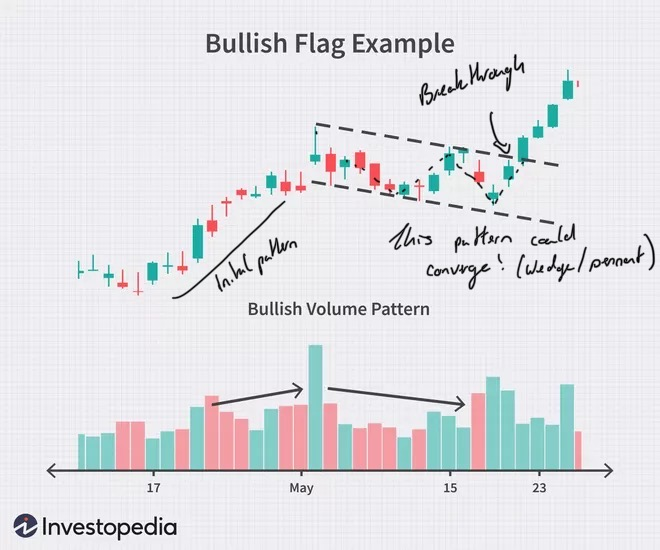
\includegraphics[width=1\columnwidth]{flag.jpg} % Example image
	\caption{Flag example}
\end{figure}

Price pattern that moves counter to the prevailing price trend, it can be recapturing a previous
trend. Generally shown over 5\-20 bars. \\

Flags have parallel markers (resistance and support lines) formed via the trend, they can also
form a wedge or pennant, a converging trend is considered more reliable as displays a the last
moments of a previous trend.\\

Strong volume before the range bars and following the breakthrough are good indicators of success.

\subsection{What are Keltner Channels ?}

Volatility based bands, placed on either side of an the EMA (generally 20 day period) determines trend.

Breaks above or below the channel of the current price showing a continuation, as the Keltner channer
shows the current Volatility and breaking through signifies a new stronger trend.

Made of three lines:
\begin{itemize}
	\item Middle line: EMA
	\item Upper line : EMA + 2 ATR
	\item Lower line:  EMA - 2 ATR
\end{itemize}

Increasing the period of the EMA or ATR will increase the lag of the indicator.\\

The factor on the ATR can be adjusted as wanted on the EMA.

\subsection{What are boiler bands ?}

The same concept as Keltner channels except use STD instead of ATR.


\subsection{What is the Diamond Top Formation ?}

A off center pushed to the left side head position with two shoulder points and a bounce in between
the head and shoulders. Connected with the low point give a diamond shape. Diamond is extended to give
the support and resistance lines.

\begin{figure}[h] % [h] forces the figure to be output where it is defined in the code (it suppresses floating)
	\centering
	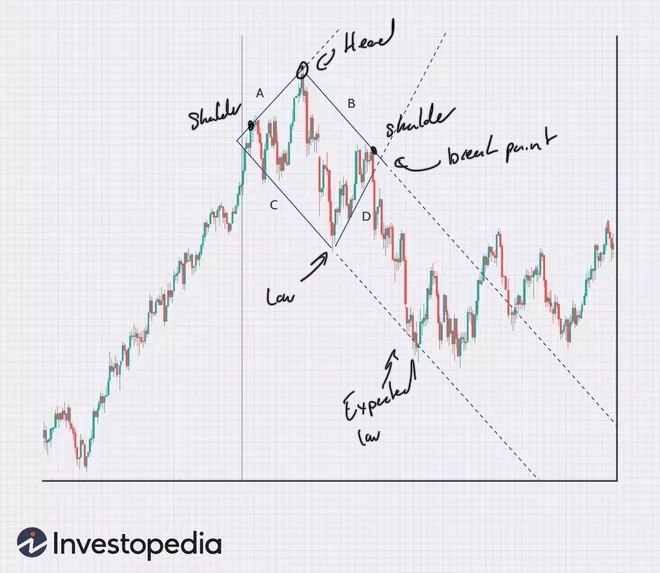
\includegraphics[width=1\columnwidth]{Diamond Top Formation .jpg} % Example image
	\caption{Diamond Top example}
\end{figure}

The break point is used to set a short position with the expected low as the stop loss.

\subsection{What is the Pennant ?}

Shows a significant expected swing in momentum, a pattern converges on trend lines.

The pattern shows a period of consolidation then a significant breakout. The volume of the consolidation
should be lower than the breakout.

\begin{figure}[h] % [h] forces the figure to be output where it is defined in the code (it suppresses floating)
	\centering
	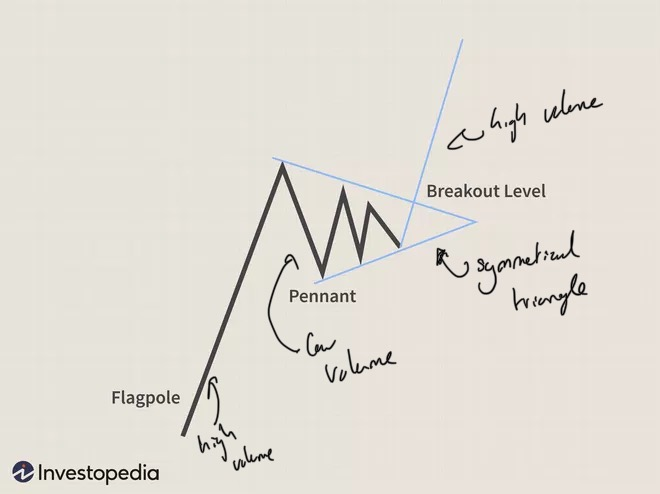
\includegraphics[width=1\columnwidth]{Pennant3.jpg} % Example image
	\caption{Pennant example}
\end{figure}

\begin{itemize}
	\item Set long position on the resistance line 
	\item Set stop loss at the lowest point on the pennant
\end{itemize}

\subsection{What is the Double bottom/top ?}

Follows the pattern: Drop, rebound, drop, rebound.

\begin{figure}[h] % [h] forces the figure to be output where it is defined in the code (it suppresses floating)
	\centering
	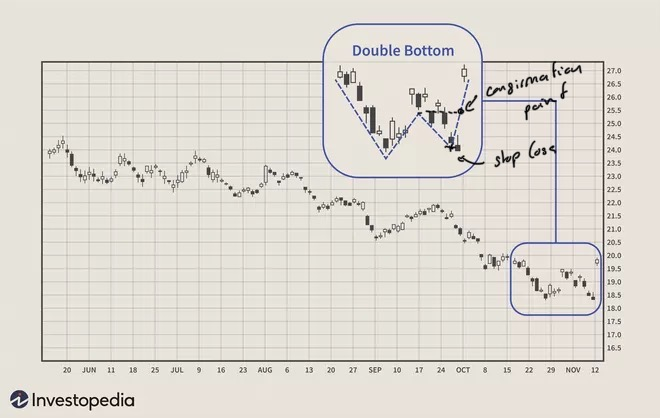
\includegraphics[width=1\columnwidth]{DoubleBottomDefinition2.jpg} % Example image
	\caption{Double Bottom example}
\end{figure}

The Double top is the same but reversed.

\section{Fibonacci tools}

Fibonacci series is present regularly in nature, a series of number created from the addition of the
previous two, with two numbers next to each other divided tending towards the golden ratio as the 
series continues. The golden ratio a irrational number being 1.68.

Based on the idea mass psychology trends towards the given by the Fibonacci series.

\subsection{Timezones}

After an initial swing the x axis, at the start of the swing + points on the series gives the zones,
in which another swing is likely.

Normally start at 13 on the series as the first number are clustered.

\subsection{Retracement/Extension}

Horizontal lines on a chosen base line (high and low) at 23.6,38.2,50,61.8,78.6\%.

\section{Metrics}

\subsection{What is delta ?}

Delta is the difference between number of buyers at ask price and number of sellers at bid price.

\[ Delta = Volume\:of\:transactions\:at\:ask\:price - volume\:of\:transactions\:at\:bid\:price \]

This shows the strength of the buyers and sellers (if >0 Stronger buying pressure, if <0 stronger 
selling pressure)

\subsubsection{What is cumlative delta ?}

This delta summed.

\subsubsection{What happens when delta and price diverge ?}

If the price hits a new high and cum delta does not this signals buyers are exhausted and sell pressure will
push down the price with a sell off. Vice versa.

\subsection{What is a stochastic Oscillator ?}

This is a value between 0-100 (Oscillator) that confirms a trends reversal.

\[ K(\%) = ((Close price - low) \div (High price - Low price)) * 100\] 

This shows how close the current price is to the max price historical price width (orientated towards the low).
At 100 the current price is the same as the max width, showing a new high is about to be hit.

Advised to exit strat at 80 or 20 as breakthrough are a rare occurrence due to market psychology pushing
against these barriers.\\

This can be tuned to your chosen period of time to determine the high and low price.

\subsection{What is the Relative Strength Index?}

A measure of the speed and magnitude of securities price changes. An Oscillator (0-100).

Shows undervalued and overvalued conditions.\\

70 is considered overbought (Bearish)
30 is considered undersold (Bullish)

\[ RSI_{step-one} = 100 - (\frac{100}{1+\frac{aveage gain}{aveage loss}}) \]

Average gain is over a chosen period of days, with any days with loss not included. And vice versa

\[ RSI_{step-two} = 100 - (\frac{100}{1+ \frac{\Sigma avergegain}{\Sigma averge loss}}) \]
The sum is over 14 periods of chosen average period.\\

Measure of gain to loss ratio, standardized between 0-100 and smoothed over many periods. At 100 x gain to loss RSI step one would become 100.

\subsection{What is True Strength Index (TSI)?}



\subsection{MACD (Moving Average Convergence Divergence)}

\[ MACD = 12\:day\:EMA - 24\:day\:EMA \] 

\textbf{EMA:} Exponential moving average (average price weighted for most recent values)

9 day EMA of the MACD is the signal line.\\

THE MACD shows clearly any new trends as the EMAs diverge, there must be a new trend emerging. The 
more they diverge the stronger the trend.\\

MACD below the signal line is bearish and above is bullish. MACD also will pivot about 0 which is a sign
of bull or bear. At 0 shows the market is stable.

\subsection{EMA Exponential moving average}

\[ EMA = Value_{today} *(\frac{smoothing}{1 + days}) + EMA_{yesterday}*(1-\frac{Smoothing}{1+days}) \]

days: Days in EMA.\\

As the days increase the weighting is reduced for the newest day.\\

To calculate the first EMA use SMA.

\subsubsection{What is double EMA ?}

\[ DEMA = 2*EMA - EMA(EMA) \]

\subsection{What is the PPO ?}

The percentage price oscillator (PPO) :

\[ PPO = \frac{12\:period\:EMA - 26\:period\:EMA}{26\:period\:EMA} *100 \]

Diff of EMAs as a ratio of 26 period EMA, shows relatively how strong the recent trend is ie 100 would
show the 12 day period is double the 26 day. Relative value of MACD compared to previous 26 days.

\section{Bid Ask Spread}

Two player in the market: price trader and market maker.\\

The market maker will offer selling (ask price) and the buy (at the bid price).\\

A trader will buy at the ask price and sell at the bid price. The difference between these is the
spread.\\

SPREAD = ASK - BID (cost of trading)

Brokerages make money crossing the trade.\\

The size of the spread represents supply and demand, as one side moves this reflects these two factors
changing. Increased spread means a decrease in liquidity, ie currency is very liquid and has a small spread.

\[ Spread(\%) = spread \div lowest asking price \]

\subsection{What is ATR (Average True Range)}

An average of the "true range" over a number of periods (generally 14 days)

"true range" = TR

\[ TR = MAX((High-Low),(High - Price\:Close),(Low-Price\:Close)) \]

The ATR shows volatility, a high value means high volatility and a low value shows low volatility.

\section{What is the Elliot wave theory ?}

\begin{figure}[t] % [h] forces the figure to be output where it is defined in the code (it suppresses floating)
	\centering
	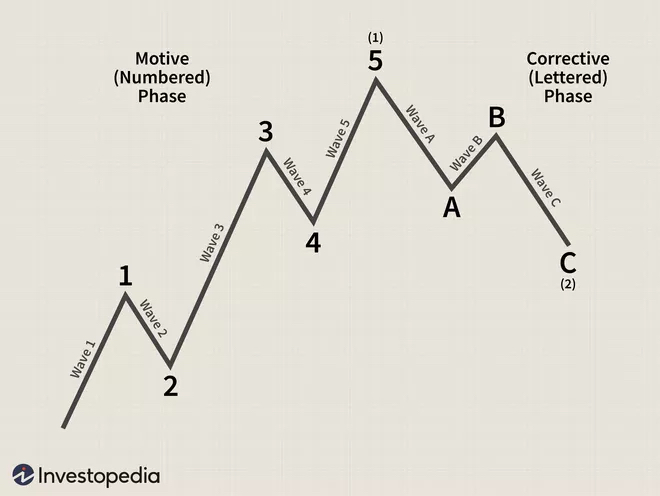
\includegraphics[width=0.8\columnwidth]{ElliottWaveTheory.jpg} % Example image
	\caption{Elliot Wave}
\end{figure}

Uses wave like patterns to predict price, two types of waves: motive (impulse) and corrective waves.

The concept is regularly you are able to find similar waves patterns in markets, this being
a fractal pattern.

\subsection{What are the rules ?}

\begin{itemize}
	\item Wave 2 cannot be greater than wave 1
	\item Wav 3 must be greater than wave 1 and wave 5
	\item Wave 4 should be smaller than wave 3
\end{itemize}

\section{Candle Patterns}

Candles show how much an asset has moved over a period of time. 

\begin{figure}[t] % [h] forces the figure to be output where it is defined in the code (it suppresses floating)
	\centering
	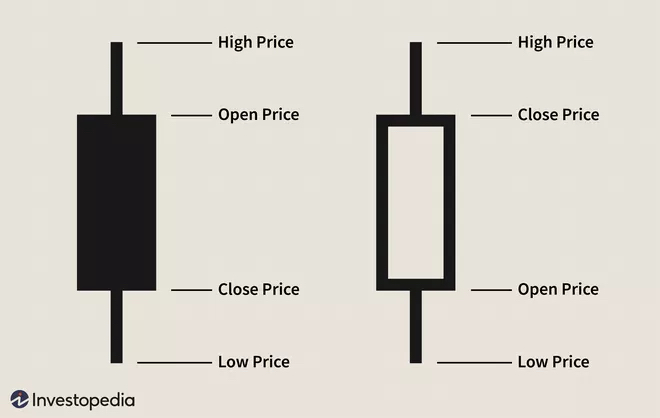
\includegraphics[width=0.8\columnwidth]{UnderstandingBasicCandlestickCharts.jpg} % Example image
	\caption{Candles}
\end{figure}

The body shows how much a price has moved over said period of time from the opening price to the 
closing. The wicks shows the over that period of time the highest and lowest prices, 
these two in conjunction can represent trends.

\begin{itemize}
	\item Long wick above shows significant sales (Bearish)
	\item Long wick below shows significant buys (Bullish)
\end{itemize}

A series of set candle patterns indicate price movements, trends and momentum.

\subsection{Bearish engulfing pattern}

Small positive prices increase (generally green) engulfed by large negative price decrease 
(generally red). 

**Indicates sellers are back in control, trend will be prices continuing to decline**

\subsection{Bullish engulfing pattern}

Opposite pattern of bearish.

\subsection{Evening star} 

Change in price direction with a larger body than previous.

Bear/Bullish depending on direction, indicates continuation in the new direction.

\subsection{Harami}

If there is a change in price direction in with a smaller body than previous, indicates potential 
predictable movements.

\subsection{Rising Three}

Consecutive days of opposite movement within the last body then a change with a larger body of the 
previous. Despite a movement for a period of time downward, indicates a new bullish movement.

\subsection{Hammer}

Bullish trend with a downward trend followed by a candle with a small body and long bottom wick.

Inverse hammer has instead a long top wick.

Bearish trend is the same pattern but starts with a upward trend.

\subsection{Three white soldiers}

Upward trending three solid candle bodies with a continued positive trend, is Bullish.

Same for bearish but a downward trend.

\subsection{Falling/Rising three}

Three solid bodies in the opposite of the previous and following trend. Good indicator the previous
trend is strong.

\section{Other}

\subsubsection{What is the Breakeven Point?}

\[ BP = Fixed costs \div (Rev - var costs) per unit \]

BP shows the number of units needed to break even.

\subsubsection{What is a cross trade ?}

Buy and sell an asset with a report of the trade by the broker after the trade is made. \\

%----------------------------------------------------------------------------------------
%	FIGURE EXAMPLE
%----------------------------------------------------------------------------------------

% \begin{figure}[h] % [h] forces the figure to be output where it is defined in the code (it suppresses floating)
% 	\centering
% 	\includegraphics[width=1\columnwidth]{IMAGE_NAME.jpg} % Example image
% 	\caption{European swallow.}
% \end{figure}

%----------------------------------------------------------------------------------------
% MATH EXAMPLES
%----------------------------------------------------------------------------------------

% \begin{align} 
% 	\label{eq:bayes}
% 	\begin{split}
% 		P(A|B) = \frac{P(B|A)P(A)}{P(B)}
% 	\end{split}					
% \end{align}

%----------------------------------------------------------------------------------------
%	LIST EXAMPLES
%----------------------------------------------------------------------------------------

% \begin{itemize}
% 	\item First item in a list 
% 		\begin{itemize}
% 		\item First item in a list 
% 			\begin{itemize}
% 			\item First item in a list 
% 			\item Second item in a list 
% 			\end{itemize}
% 		\item Second item in a list 
% 		\end{itemize}
% 	\item Second item in a list 
% \end{itemize}

%------------------------------------------------

% \subsection{Numbered List}

% \begin{enumerate}
% 	\item First item in a list 
% 	\item Second item in a list 
% 	\item Third item in a list
% \end{enumerate}

%----------------------------------------------------------------------------------------
%	TABLE EXAMPLE
%----------------------------------------------------------------------------------------

% \section{Interpreting a Table}

% \begin{table}[h] % [h] forces the table to be output where it is defined in the code (it suppresses floating)
% 	\centering % Centre the table
% 	\begin{tabular}{l l l}
% 		\toprule
% 		\textit{Per 50g} & \textbf{Pork} & \textbf{Soy} \\
% 		\midrule
% 		Energy & 760kJ & 538kJ\\
% 		Protein & 7.0g & 9.3g\\
% 		\bottomrule
% 	\end{tabular}
% 	\caption{Sausage nutrition.}
% \end{table}

%----------------------------------------------------------------------------------------
%	CODE LISTING EXAMPLE
%----------------------------------------------------------------------------------------

% \begin{lstlisting}[
% 	caption= Macro definition, % Caption above the listing
% 	language=python, % Use Julia functions/syntax highlighting
% 	frame=single, % Frame around the code listing
% 	showstringspaces=false, % Don't put marks in string spaces
% 	numbers=left, % Line numbers on left
% 	numberstyle=\large, % Line numbers styling
% 	]

% 	CODE

% \end{lstlisting}

%----------------------------------------------------------------------------------------
%	CODE LISTING FILE EXAMPLE
%----------------------------------------------------------------------------------------

% \lstinputlisting[
% 	caption=Luftballons Perl Script., % Caption above the listing
% 	label=lst:luftballons, % Label for referencing this listing
% 	language=Perl, % Use Perl functions/syntax highlighting
% 	frame=single, % Frame around the code listing
% 	showstringspaces=false, % Don't put marks in string spaces
% 	numbers=left, % Line numbers on left
% 	numberstyle=\tiny, % Line numbers styling
% 	]{luftballons.pl}

%------------------------------------------------

\end{document}